% Template v2.0: 11/13/2018.   The previous template is also acceptable. 
% Template for white paper submissions for the 
% LSST Call for Observing Strategies for DeepDrilling and Minisurveys 
% 
% The call for white papers can be found at https://github.com/lsst-pst/survey_strategy/blob/master/latex/WPcall2018.pdf
% The deadline for submissions is November 30, 2018
% To submit white papers, please email the compiled PDF to lsst-survey-strategy@lists.lsst.org   
%  OR submit a pull request to this github repository (github.com/lsst-pst/survey_strategy_wp) with your white paper in a clearly named subdirectory.
% For help with white papers or the submission process, please post at http://community.lsst.org/c/sci/survey-strategy


\documentclass[12pt, letterpaper]{article}
\usepackage[top=1in, bottom=1.5in, left=1in, right=1in]{geometry}
\usepackage[utf8]{inputenc}
\usepackage{booktabs}
\usepackage{hyperref}
\usepackage[square,numbers,sort&compress]{natbib}

\usepackage[english]{babel}
\usepackage{amsmath}
\usepackage{amssymb}
\usepackage{graphicx}
\usepackage{hyperref}
\usepackage{wrapfig,verbatim,caption,subcaption,calc,relsize,multicol,enumitem,titlesec}

\usepackage[utf8]{inputenc}
\usepackage{booktabs}
\usepackage[utf8]{inputenc}
\usepackage{natbib}
\usepackage{color}

%Includes "References" in the table of contents
\usepackage[nottoc]{tocbibind}
\def\apj{AstroPhysical Journal}             % Astrophysical Journal
\def\apjl{Astrophysical Journal, Letters}                % Astrophysical Journal, Letters
\def\apjs{Astrophysical Journal, Supplements}  \def\nat{Nature}               % 
\def\mnras{Monthly Notices of the Royal Astronomical Society}
\newcommand\mathmacro[1][A]{\ensuremath{{#1}_1}}

%%% macroe %%%
\newcommand{\dtone}{\ensuremath{\Delta T_1}}
\newcommand{\dttwo}{\ensuremath{\Delta T_2}}
\newcommand\rahul[1]{\textcolor{blue}{#1}}

\title{{\em Presto-Color:} An LSST Cadence for \\ Explosive Physics \& Fast Transients}
\author{\small{Federica B. Bianco\footnote{fbianco@nyu.edu}, New York Univeristy CUSP/CCPP, University of Delaware;}\\\small{Melissa Graham, University of Washington;}\\\small{Maria R. Drout, University of Toronto, Carnegie Observatories;}\\\small{Igor Andreoni, Caltech; Rahul Biswas, Stockholm University; Philip Cowperthwaite,}\\\small{Carnegie; Gautham Narayan, STScI; Tyler A. Pritchard, NYU; Tiago Ribeiro, LSST;}}
%Affiliation: "The Oskar Klein Centre for CosmoParticle Physics, Department of Physics, Stockholm University, AlbaNova, Stockholm SE-10691"\date{\today}

\begin{document}
\maketitle
\vspace{-0.3in}
\begin{abstract}
We propose a cadence for the LSST survey in which three visits are obtained per night: two different filters within a short time window (e.g., $g$ \& $i$ or $r$ \& $z$ within $<0.5$ hours) and a repeat of one of those filters with a longer time window (e.g., $>1.5$ hours). We colloquially refer to this as the {\em Presto-Color} strategy (quick-color). This observing strategy delivers both the color and lightcurve evolution of transients on the same night. This will enable us to identify and characterize fast transients -- or fast features of longer timescale transients -- such as rapidly-declining supernovae (SNe), kilonovae (KNe), and the signatures of SN ejecta interacting with binary companion stars or circumstellar material. Such extragalactic transients are intrinsically rare, thus LSST could dramatically improve our understanding of their origin and properties. This cadence can be implemented as a Mini-Survey or as part of a Wide-Fast-Deep survey on selected portions of the extragalactic sky.
\end{abstract}

\section{White Paper Information}
\begin{enumerate} 
\vspace{-0.05in}
\item {\bf Science Category:} Exploring the Transient Sky, Dark Energy \label{sec:item:category}
\vspace{-0.05in}
\item {\bf Survey Type Category:} We are proposing this cadence as a variation of the  ``Wide-Fast-Deep" (WFD) Main Survey, but it could also be considered for implementation as a Mini-Survey or a Deep Drilling Field, and done in only a portion of the sky. 
\vspace{-0.05in}
\item {\bf Observing Strategy Category:} This is an observing strategy to enable specific time domain science, which is relatively agnostic to where the telescope is pointed. 
\end{enumerate}  


\clearpage
%%%%%%%%%%%%%%%%%%%%%%%%%%%%%%%%%%%%%%%%%%%%%%%%%%%
\section{Scientific Motivation}

The advent of wide-field time domain surveys has revolutionized the field of transient astrophysics. Coverage on \emph{short timescales}, in particular, has facilitated rapid strides in our understanding of both supernova (SN) explosions and peculiar transients. Observations of ``infant'' SN---obtained hours to days after explosion---evolve quickly and provide vital constraints on their explosion mechanisms and progenitor systems. The emission at these epochs contains natal information about the progenitor characteristics \citep{Nakar2010,Rabinak2011,Nugent2011}, potential non-spherical behavior \citep{Matzner2013,Salbi2014}, and shock collision with a binary companion \citep{Kasen2010}. In addition, rapidly-evolving transients ($\lesssim$10 days) may be associated with a variety of poorly-understood events, including accretion-induced white dwarf collapse \citep{Metzger2009}, underluminous and fallback SN~\citep{Moriya2010}, ultra-stripped SN \citep{Drout2013,Kasliwal2010,Tauris2015}, compact-object mergers \citep{Kasen2015,Metzger2010}, orphan GRB afterglows \citep{Totani2002}, and common-envelope ejections \citep{Blagorodnova2017}.

%Do need to emphasize a bit about rates, or make it clear that 
%Need to mention ''fast features'' somewhere. They use that language. 

Despite progress, the detection rate for both rapid transients and rapidly-evolving \emph{phases} in SN explosions has remained low---due to a combination of survey efficiency and intrinsic event rates. The volume surveyed by LSST brings the promise of detecting many more intrinsically rare events. However, \emph{using} these events to probe the science questions described herein requires adequate time- and filter-sampling of relatively short-lived events---sampling that will \emph{not} be achieved through the WFD survey alone. Thus, we require a cadence that allows us to effectively \emph{recognize} young and rapidly-evolving transients from within millions of LSST alerts in order to trigger additional follow-up. Such a cadence has two requirements: 
\begin{enumerate}
    \item Observations in {\bf two filters} obtained in quick succession so that {\bf color} can be measured. This is critical to both allow us to distinguish different classes of transients and as a probe of the physics operating during these phases.
    \vspace{-0.1in}
    \item A {\bf same-filter} revisit separated by hours (before/after the filter pair) so the lightcurve {\bf behaviour/slope} can be analyzed and distinguished from slower-evolving transients.
\end{enumerate}
%(1)~observations in two filters obtained in quick succession so that color can be measured, and (2)~a same-filter revisit within hours so the lightcurve behaviour can be analyzed and distinguished from slower-evolving transients. 

%More information on each of these: 
%Light curve rise critical to distinguish from standard SN.
%Color: critical for initial classification.

As we will show, the WFD baseline survey's inter-night revisit rate of once every 10-20 nights (in the same filter) is too sparse, and the intra-night revisit rate of $\sim$30 minutes is too rapid, to detect \emph{and recognize} fast transients/phases. The exact form of our proposed cadence is given in Section 3. In order to define our diagnostics we have selected four exemplar types of extragalactic fast transients/features. Representative light curves for each type of transient are shown in Figure~1, and graphical representations of where they separate from normal SN in color and intra-night rate-of-change are shown in Figure 2. Main science cases are discussed below.
%basic color and rate-of-change information are provided in Table 1,
\smallskip


%\smallskip

\noindent {\bf I. The Nature of Rapidly-Evolving Luminous Transients:} ``Rapidly-evolving transients'' are defined as extragalactic events that reach SN luminosities but have timescales an order of magnitude faster. To date, only a small number have been identified, but recent systematic studies \citep{Drout2014} have shown that they are not \emph{intrinsically} rare---few have been detected simply because surveys were not designed to be efficient at short timescales. They represent a significant channel ($\sim$5--10\% of the core-collapse rate) which we must understand to have a complete picture of stellar death. Known events have rise times spanning 1--3 days and blue colors at maximum \citep{Drout2014,Pirsiainen2018,Rest2018}. While their true nature is unknown, leading theoretical models range from black hole formation in failed SN to the birth of binary neutron star systems, with recent observations of AT2018cow show evidence for a central engine \citep{Kashiyama2015,Prentice2018,Margutti2018}. %More observations are required to understand their true nature and diversity. 
%They are luminous, blue, 

%More events are required to determine the nature and 
%However, these transients .

% [10,11,30], but recent studies [31] have shown that they are not \emph{intrinsically} rare---few have been detected simply because previous surveys were not designed to be efficient at short timescales. 
%with leading theoretical models including black hole formation and the birth of binary neutron star systems [5-8]

\smallskip
\noindent {\bf II. Kilonovae and the Origin of Heavy Elements:} 
Kilonova (KN) are produced by the radioactive decay of r-process nuclei synthesized in the ejecta of neutron star mergers \citep{Li1998}.  Observations of the KN associated with GW170817 revealed thermal emission that rose in $<$1 day and cooled from a temperature of $>$10,000K to 3,000K over 5 days \citep{Drout2017}. The initially blue optical light faded at a rate of $>$1 mag/day, and was followed by a longer-lived red transient---consistent with the production of a significant quantity of of r-process elements of \emph{multiple} compositions \citep{Drout2017,Villar2017,Tanvir2017,Smartt2017,Kasliwal2017}.  Additional examples---with or without associated LIGO triggers---are required to ascertain the ``typicalness'' of GW170817, with the frequency of early blue emission providing critical constraints on the ratio of light and heavy elements formed, and the total contribution of NS mergers to cosmic nucleosynthesis \citep{Rosswog2018,Piro2018,Metzger2018}. 
%Ejecta composition and quantity strongly influences the resulting \emph{color}, \emph{magnitude}, and \emph{timescale} of the emission.
%thermal emission that rose in $<$ 1 day and cooled from a temperature of $>$10,000K to 3,000K over 5 days, followed by a longer-lived IR transient [X]
%thermal emission that rose in $<$ 1 day and cooled from a temperature of $>$10,000K to 3,000K over 5 days

\smallskip
\noindent {\bf III. Progenitors and Pre-explosion Mass Loss of Core-Collapse SN:} Early observations of core-collapse SN (CCSN) provide critical constraints on the progenitor radius and envelope structure through the detection of either shock breakout ($\sim$1 day) or cooling envelope ($\sim$1-5 day) emission \citep{Nakar2010,Arcavi2011,Bersten2018}. Indeed, there has been growing evidence that many CCSN either explode in ``non-standard'' evolutionary states or undergo enhanced pre-SN mass-loss and outbursts in their terminal years \citep{Khazov2016,Nakar2014}. Theoretical studies have pointed to a range of potential explanations to accommodate the observations, such as pulsation-driven superwinds \citep{Yoon2010}, wave heating outbursts \citep{Fuller2017}, and inflated progenitor envelope \citep{Grafener2012}. However, the nature of this mass loss and the types of SN experiencing it remain uncertain.



\smallskip
\noindent {\bf IV. Progenitors and Explosion Mechanisms of Thermonuclear SN:}
Type Ia SN result from the thermonuclear disruption of a CO white dwarf \citep{Hillebrandt2000}. However, questions remain regarding the nature of their binary companions. Recently, observations of SN2017cbv obtained within $\sim$1 day of explosion revealed a rapidly-rising blue ``bump'', interpreted by some as a collision with a non-degenerate companion \citep{Hosseinzadeh2017}. At the same time preliminary population studies reveal an as-yet-unexplained red/blue color dichotomy in the early ($<$ 5 days) rapidly-rising light curves of Type Ia SN \citep{Stritzinger2018}, with implications for outwardly mixed radioactive material predicted by the double detonation explosion model \citep{Piro2016,Polin2018}. Further observations are required to ascertain the nature of this early emission, with implications from stellar physics to cosmology.




\smallskip
\noindent {\bf V. Additional Science Cases:} While we have focused on extragalactic fast transients here, a cadence that allows measurement of both color and rate-of-change on the timescale of $\sim$hours will have general applicability across many areas---from variable stars and microlensing to characterization of solar system objects.

\smallskip
Finally, though we describe here an adaptation to the general WFD cadence to facilitate the timely identification of rapid events, our cadence could alternatively be adopted as a mini-survey over a portion of the sky. If coupled with a shorter intra-night cadence (as part of a mini-survey or within a rolling cadence) LSST observations alone could provide sufficient light curve coverage to probe progenitors and explosion physics of fast transients/features.

\bigskip

%\noindent {\bf MRD Note: I'm still working to clean this up and cut some text. A few things could move to later sections. Ah, we now have more room! I will expand a few things slightly and fix the references.}

\clearpage
%%%%%%%%%%%%%%%%%%%%%%%%%%%%%%%%%%%%%%%%%%%%%%%%%%%%%%%%
%%%%%ORIGINAL MOTIVATION:
%%%%%%%%%%%%%%%%%%%%%%%%%%%%%%%%%%%%%%%%%%%%%%%%%%%%%%%%%


%\begin{footnotesize}
%{\it Describe the scientific justification for this white paper in the context of your field, as well as the importance to the general program of astronomy, including the relevance over the next decade. Describe other relevant data, and justify why LSST is the best facility for these observations. (Limit: 2 pages + 1 page for figures.)}
%\end{footnotesize}

%%% MLG deleted text
% This has an especially high impact in two cases: (1) the relatively short-duration late stages of stellar evolution where the star undergoes rapid changes in the lead up to a supernova, and (2) binary (or even tertiary) systems where dynamical evolution and/or mass transfer plays a key role in determining the stellar evolutionary processes and outcomes. 

%{\bf note: the figures are place holders. original figures are in the making. the metrics described below are being written and optimal/feasible ranges for the parameters \dtone and \dttwo for different filter pairs will be investigated for a few science cases.}

%Explosive and eruptive transients that rise and fall in brightness within $3$--$5$ days have historically been rarely discovered due to sky survey efficiencies, but are also intrinsically rare ($\sim 5\%$ of the rate of core-collapse supernovae; \citealt{2014ApJ...794...23D}). Similarly, {\it fast features} in otherwise slow evolving transient events, such as ejecta impacting circumstellar material or a binary companion star in stellar explosions, are rarely caught due to their short-lived nature, and also appear to be intrinsically rare. Fast transients and fast features in transients provide a unique window on the physical mechanisms and progenitor scenarios of stellar eruptions and explosions, and the late stages of stellar evolution including mass-loss and mass-transfer in binaries.

%The volume surveyed by LSST brings the promise of finding and characterizing many more intrinsically rare events, however, adequate time- and filter-sampling of relatively short-lived events is necessary to deliver on this promise. The requisit observations in order to find \emph{and recognize} these fast events early enough to trigger follow-up, {\it and/or} characterize a large sample of fast events with LSST photometry alone, are: (1) observations in two filters obtained in quick succession so that color can be measured, and (2) a same-filter revisit within hours so the lightcurve behaviour can be analyzed. As we will show, the WFD baseline survey's inter-night revisit rate of once every three nights is too sparse, and the intra-night revisit rate of $\sim30$ minutes is too rapid, to identify (\emph{i.e.} detect and recognize) fast transients and fast features. The exact form of our proposed cadence is given in Section 3. To define our diagnostic we collect the early-time observer-frame color and rate of change of brightness for four exemplar types of extragalactic fast transients and fast features in Table 1, discuss the main science goals for each type of transient below, and provide illustrative examples in Figure 1.

%{\bf Fast Transients --} First discovered in PanSTARRs data by \cite{2014ApJ...794...23D}, also called rapidly fading supernovae (RFSNe), and thought to be driven by the shock of low-mass ejecta propagating through an extended stellar envelope or wind (e.g., \citealt{2018MNRAS.475.3152K}). There are only tens of such RFSNe discovered so far. The sample presented in \cite{2014ApJ...794...23D} mostly have $z<0.3$, rise to peak within $1$--$3$ days (e.g., PS1-10bjp rises by $2.2$ mag in $g$-band during the $2.7$ days before peak), and are optically blue (observer-frame; figure 9 of \citealt{2014ApJ...794...23D}).

%{\bf Kilonovae --} The discovery of kilonovae, whether or not they are associated with LIGO events, yeilds new insights into neutron star mergers. The optical counterpart to GW170817 presented by \cite{2017ApJ...848L..27T} shows a $<2$-day rise to peak brightness, at which point the color $r-Y\sim0.5$, after which the emission evolves redward (e.g., their figure 3) and declines quickly (e.g., $6$ mag in $\sim10$ days; their figure 2, but see also \cite{2017Natur.551...75S}). Optical data fit with theoretical models leads to contraints on the ejecta mass and velocity and the radioactive power source.

%{\bf Core Collapse Supernova Shock Breakout --} When the shock of the core collapse reaches the photosphere, high energy emission escapes in a short luminous burst (as theoretically predicted by, e.g., \citealt{1978ApJ...223L.109K}). The serendipidous discovery of nearby ($24.6$ Mpc) SN\,2016gkg's $\sim3$-day long shock-driven feature, which in it's first day exhibted a maximum rise rate of $\sim40$ $\rm mag\ day^{-1}$, is one of the best examples to date (\citealt{2018Natur.554..497B}; see also SN\,2011dh, \citealt{2011ApJ...742L..18A}). Observations of the shock breakout can directly constrain the star's radius and the mass in its envelope. While expected to be quite blue during the initial fast rise, the optical color can be neutral or even red during the $\lesssim 3$ day shock cooling phase, e.g., $B-V\sim0.5$ for SN\,2016gkg \citep[see their extended data table 3][]{2018Natur.554..497B}.
% or $g-r\sim-0.1$ for SN\,2001dh (Arcavi et al. 2011)
% by converting the g and R on the first day
% to g-r~-0.1 via Lupton (2005) http://www.sdss3.org/dr8/algorithms/sdssUBVRITransform.php#Lupton2005
% which really isn't that appropriate

%{\bf SNe\,Ia --} Blue bumps in the first hours/days of the SN\,Ia light curve are theoretically predicted to be the photometric signature of the SN\,Ia ejecta shocking a non-degenerate companion star \citep{2010ApJ...708.1025K}, and are best exemplified with observations of SN\,2017cbv by \cite{2017ApJ...845L..11H}. The values in Table \ref{tab:1} for normal and blue bump SNe\,Ia are for nearby ($<10$ Mpc) events, derived using the $UBVgri$ photometry for SN\,2017cbv and SN\,2011fe from \cite{2010ApJ...708.1025K} within the first day of observations (see their figures 1 and 2; $U-B$ is used as a substitute $g-r$, and there was no early-time $z$ or $y$ for these events). In this case, an new point source next to an elliptical galaxy rising at $>1$ $\rm mag\ day^{-1}$ with a $g-r < -0.5$ would be an excellent candidate for a blue-bump SN\,Ia and should receive immediate follow-up. %Furthermore, obtaining color and observations within the first $\sim5$ days after explosion would enable the creation of a sample able to set constraints on the fraction of SN\,Ia originating from Single Degenerate {\it vs} Double Degenerate progenitors (as done in \citealt{Bianco2011} and indicated in \citealt{COSEP} Section 6.3), with implications for stellar physics and cosmology (as SN\,Ia may follow different standardization rules for different progenitors, inducing systematics in cosmological inference).
%Furthermore, such LSST early-time photometry and color data for SNe\,Ia could be stacked over all events, and enable statistical constraints on the fraction of SNe\,Ia that exhibit blue bumps (i.e., have non-degenerate companion stars), as done by \citealt{Bianco2011} and as indicated in Section 6.3 of \citealt{COSEP}. The types of companion stars of carbon-oxygen white dwarfs that explode as SNe\,Ia has implications for stellar physics and cosmology.

% {\bf Point-Ia --} 

% {\bf IIb+CSM --}

% {\bf Accretion-Induced Collapse (AIC) --} of a white dwarf to a neutron star,  \cite{2010MNRAS.409..846D} show they last $\sim3$ days and rise within $\sim0.5$ days to a peak R-band luminosity of $10^{41}$ $\rm erg\ s^{-1}$, which is $M_R\sim -16$ mag. {\bf MLG: Fig 2 shows their color evolution.}

\clearpage

%%% MLG 11/29: Commented out table, we won't need it once Maria's new plots are integrated.
%%% MLG also removed references to this table from the text.
% \begin{footnotesize}
% \begin{center}
% \title{The early-time colors and rise rates of fast transients/features.}\label{tab:1}
% \begin{tabular}{|c|c|c|} 
% \hline
% Target Type         & $g$-band $dm/dt$ [$\rm mag\ day^{-1}$] & color [$\rm mag$] \\
% \hline 
% fast transients     & $\gtrsim-0.8$ & $g-r\leq-0.2$  \\ 
% kilonovae           & $>11$          & $r-Y\sim0.5$  \\ 
% CCSN shock breakout & $\sim-10$     & blue at $<1$ day, then neutral  \\ 
% SNIa blue bumps     & $\gtrsim -1$  & $u-g\sim-0.6$, $g-r\sim-0.2$  \\ 
% SNIa normal         & $\sim -1$     & $u-g\sim-0.2$, $g-r\sim-0.1$  \\
% %point-Ia (Bildsten) &  &  &  &  &  & \\ 
% %IIb+CSM &  &  &  &  &  & \\ 
% %AIC &  &  &  &  &  & \\ 
% \hline
% \end{tabular}
% \end{center}
% \end{footnotesize}

\begin{center}
\begin{figure}[!h]
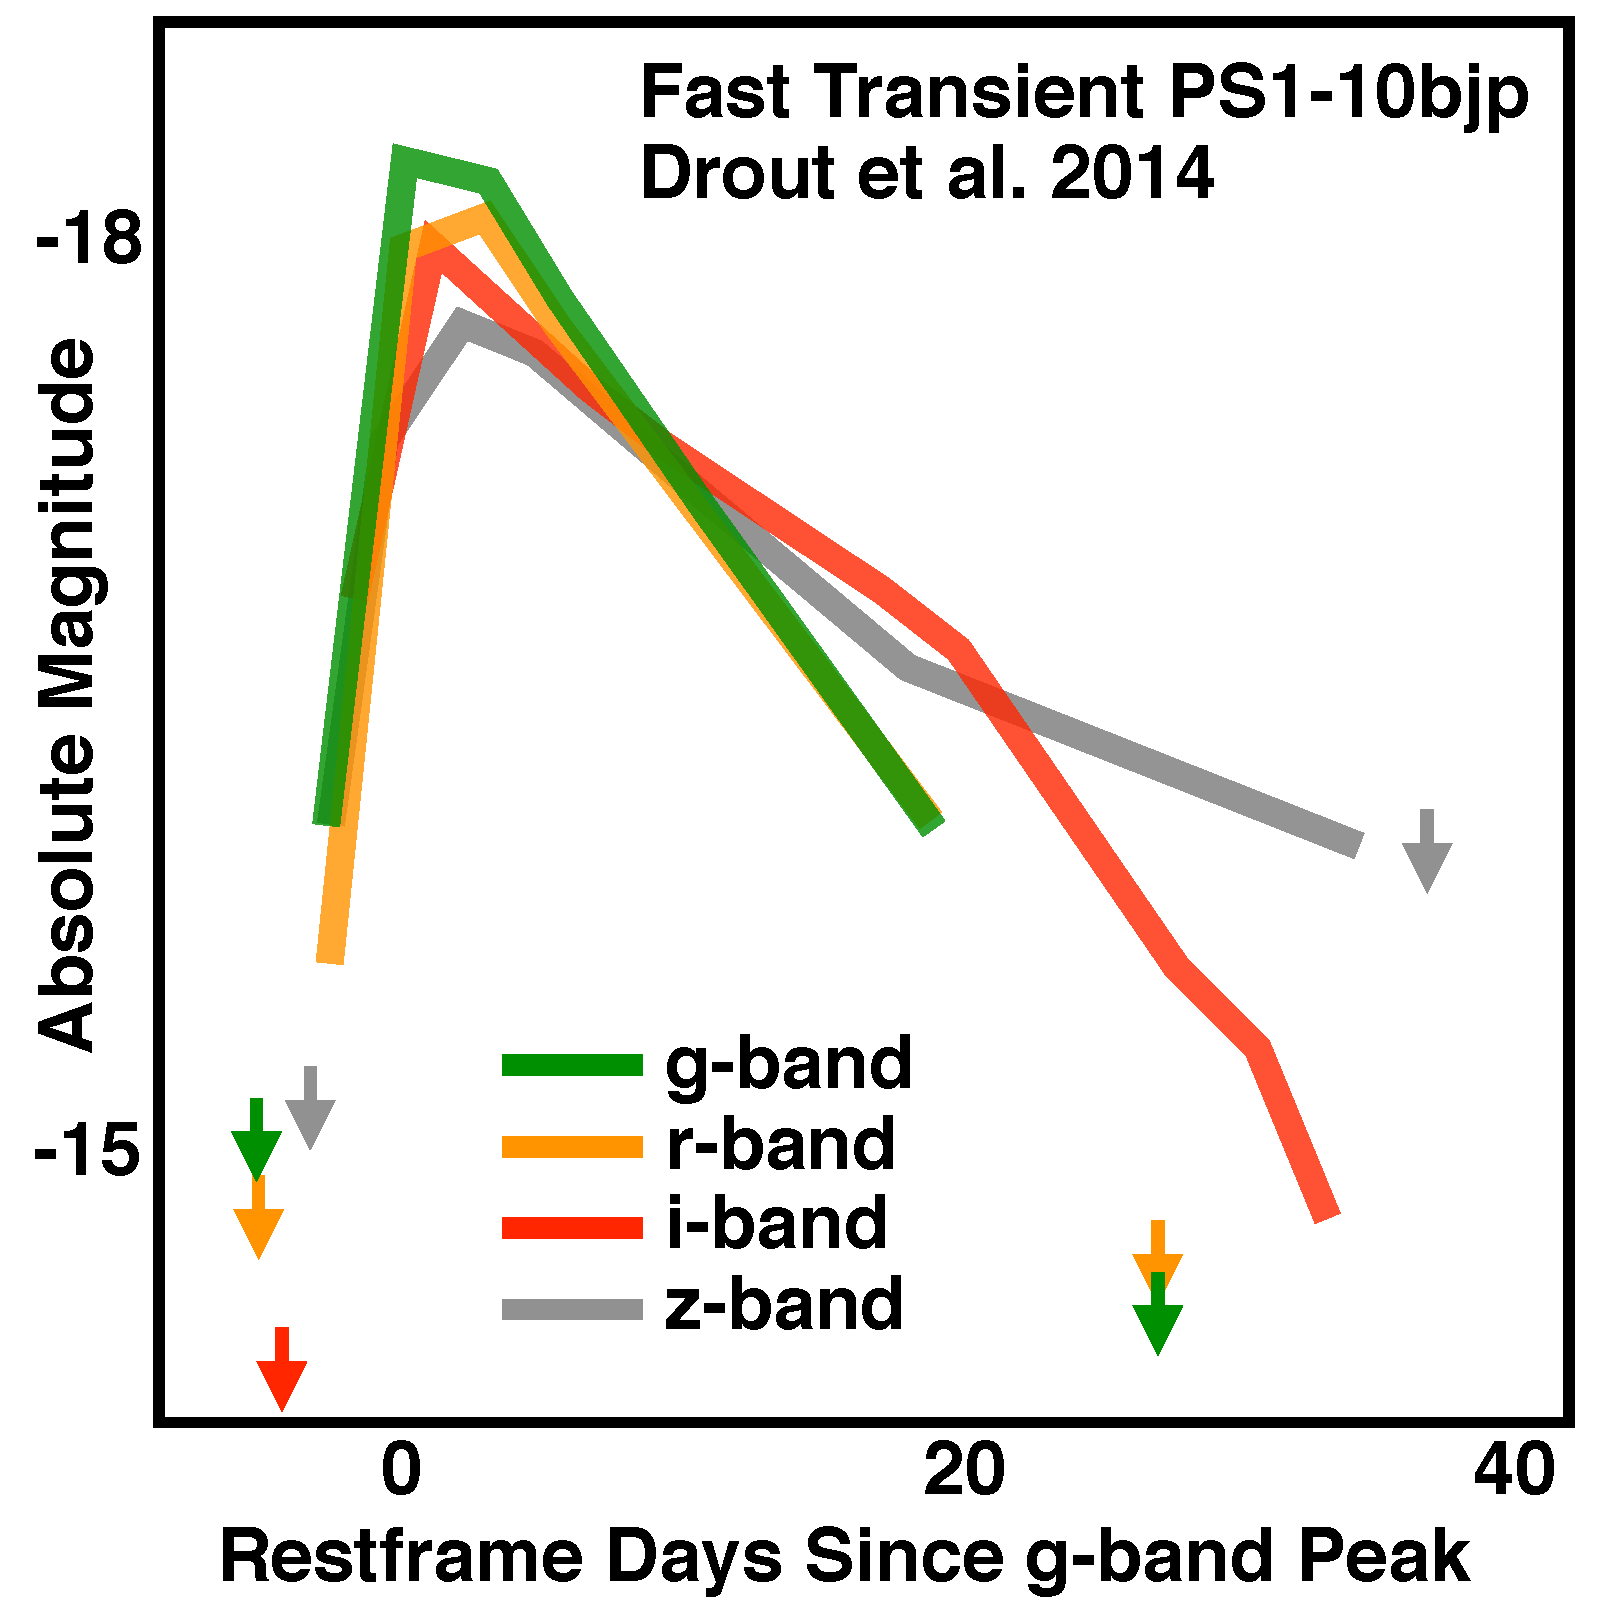
\includegraphics[width=4cm,height=4cm]{figures/fasttrans.pdf}
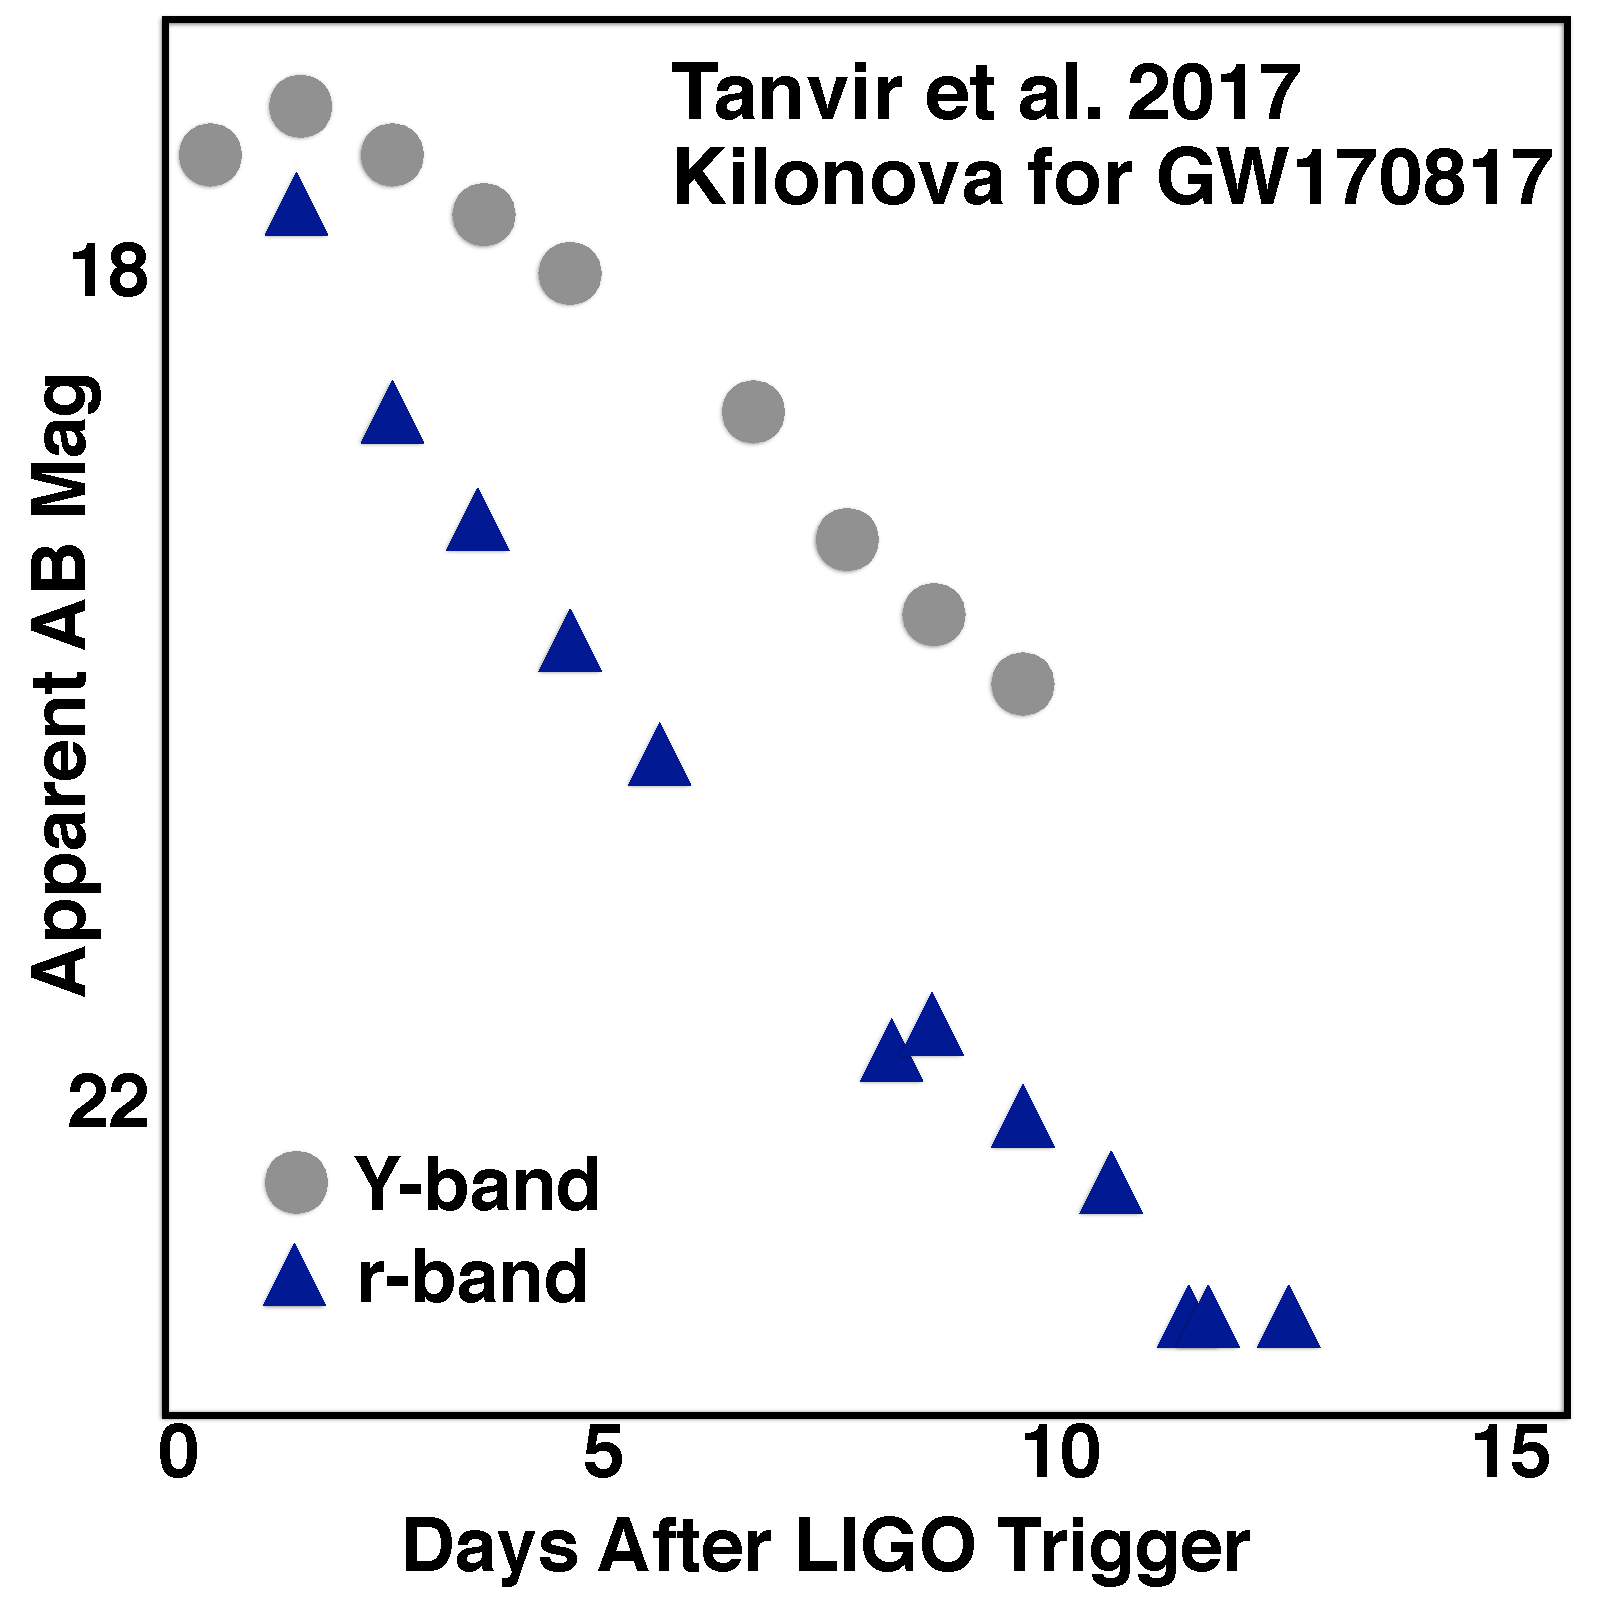
\includegraphics[width=4cm,height=4cm]{figures/Tanvir_fig2_remake.pdf}
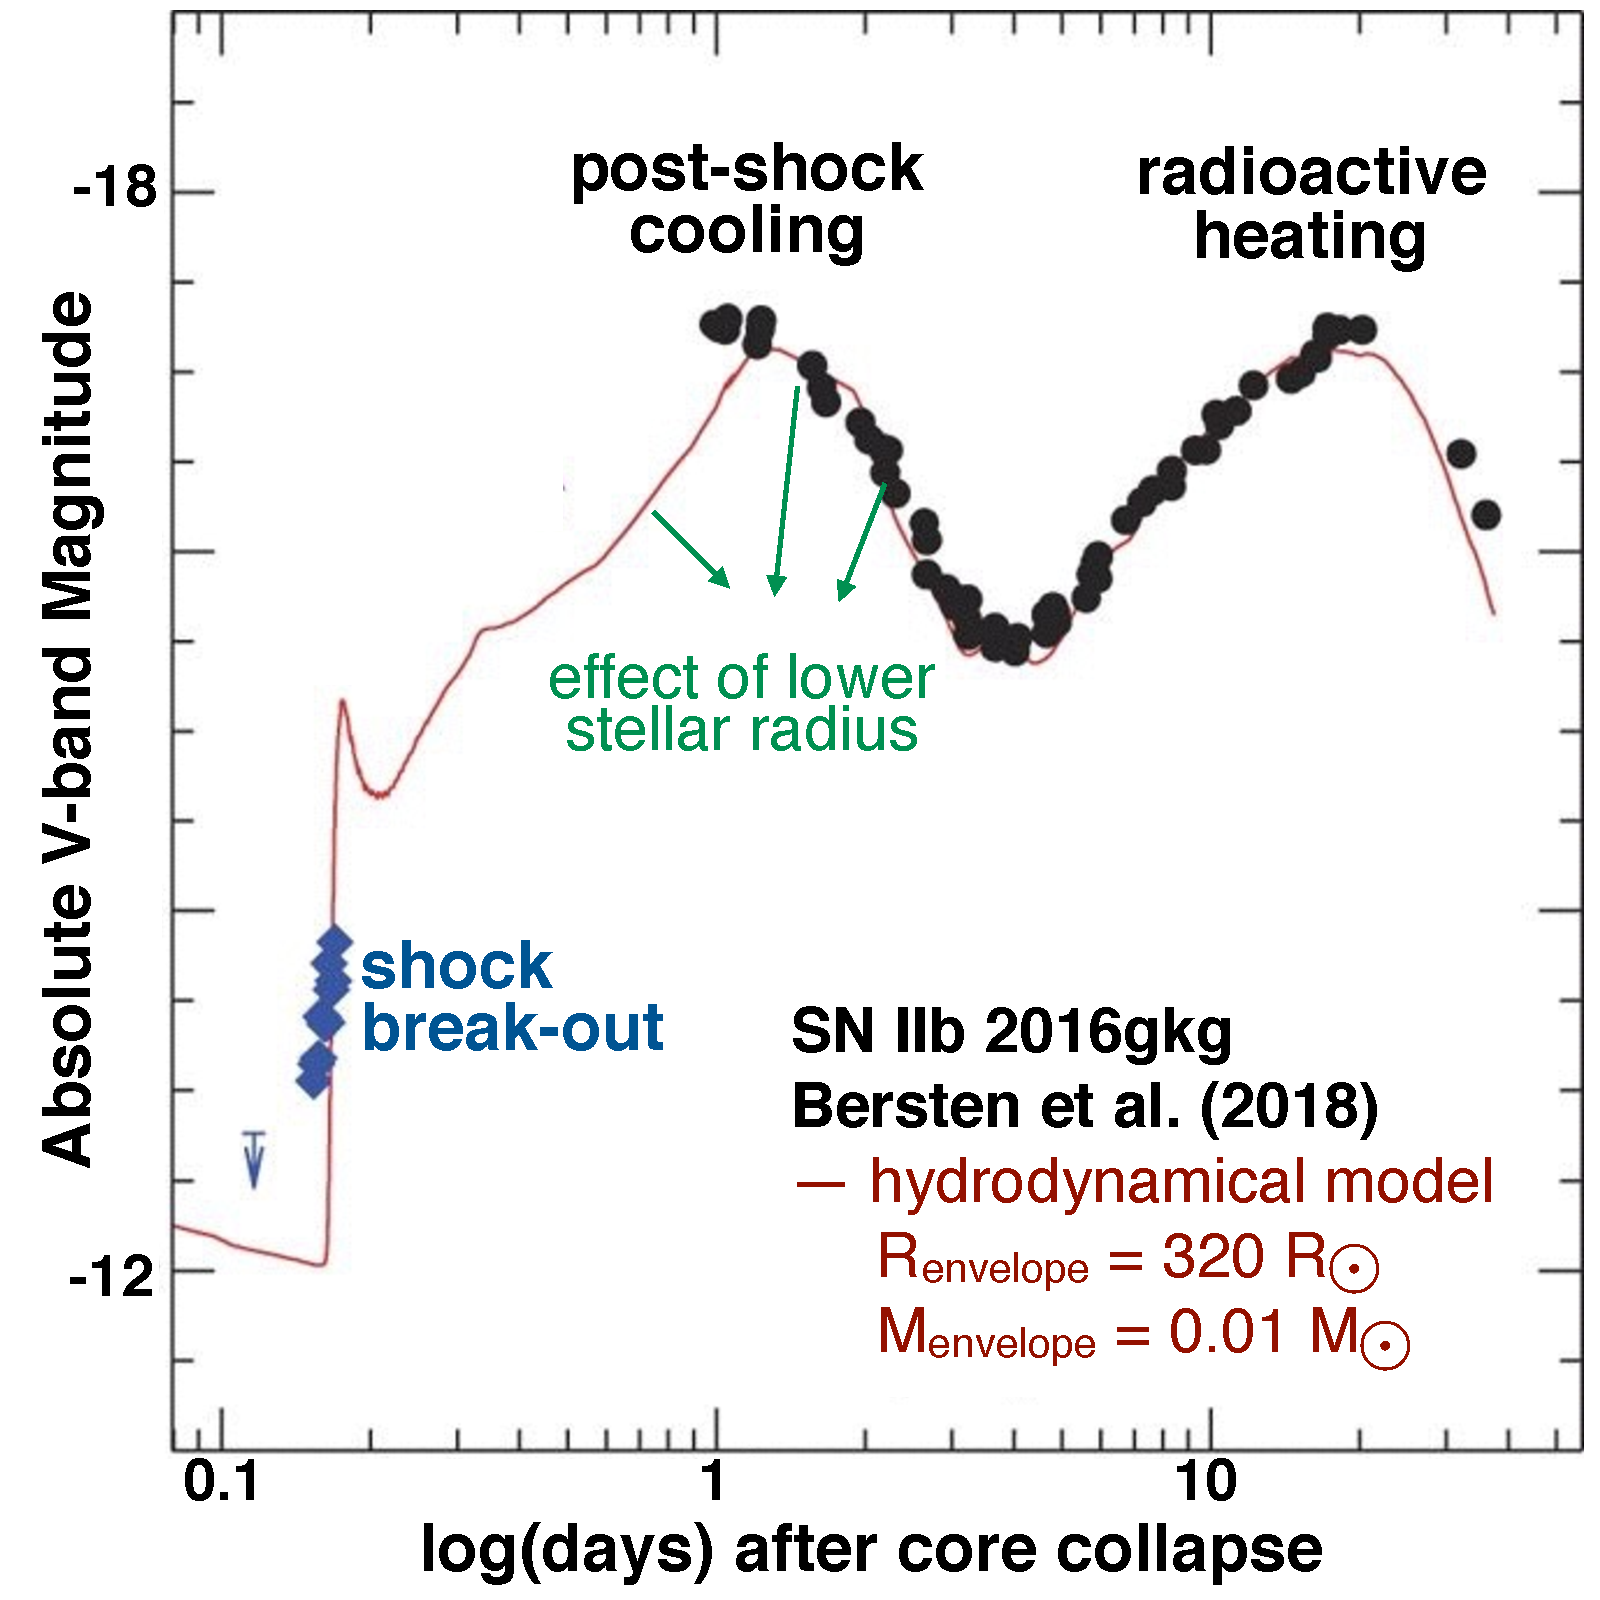
\includegraphics[width=4cm,height=4cm]{figures/2016gkg.pdf}
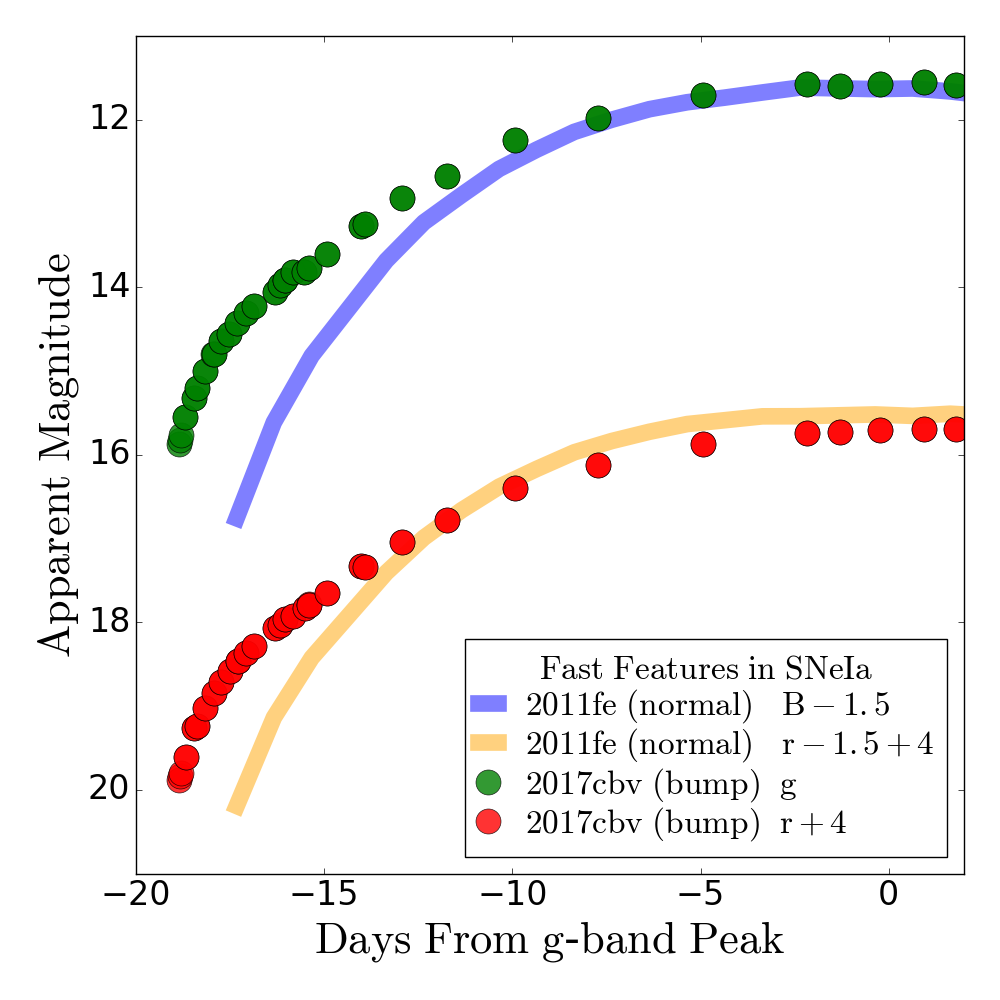
\includegraphics[width=4.2cm,height=4.2cm]{figures/bluebump.png}
\caption{{\scriptsize Light curves for our examples of fast transients and fast features. From left to right: fast transient PS1-10bjp \citep{Drout2014}; kilonova for GW170817 \citep{Tanvir2017}; the shock breakout model fits for SN\,IIb 2016gkg's stellar radius \citep{Bersten2018}; and SN\,Ia 2017cbv's blue bump compared to SN\,Ia 2011fe's ``normal" lightcurve \citep{Hosseinzadeh2017,Graham2015}.}}
\end{figure}
\end{center}


\begin{center}
\vspace{-0.5in}
\begin{figure}[!h]
\begin{center}
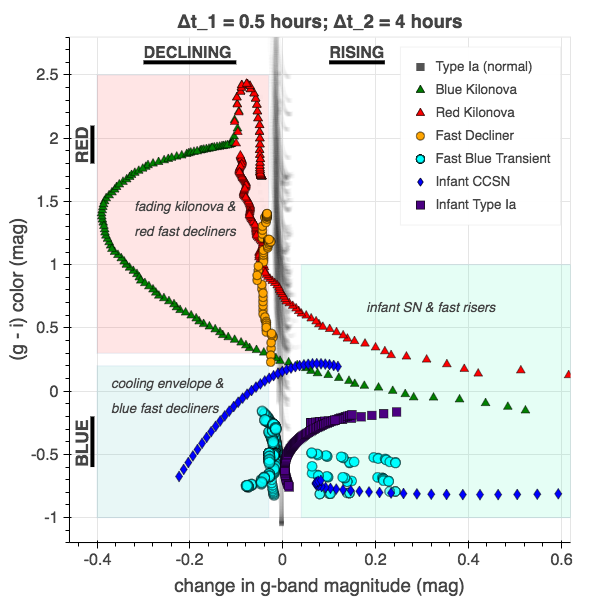
\includegraphics[height=6.5cm]{figures/LSST_PhaseSpace.png}
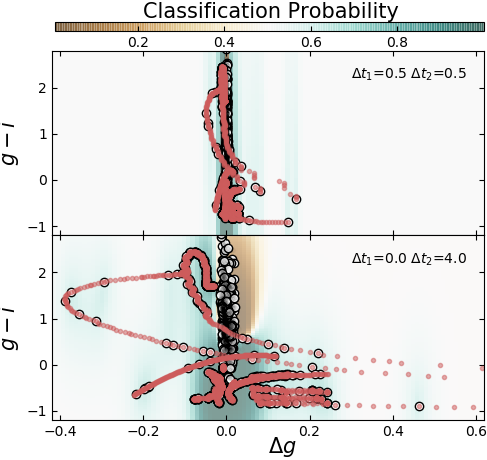
\includegraphics[height=6.5cm]{figures/FTclassifier.png}
    
\end{center}
\caption{{\scriptsize \emph{Left:} Phase space plot showing separation between classes of transients in observed color and intra-night magnitude change. This \emph{fiducial} plot assumes observations are obtained in $g-$ and $i-$band filters within 30 minutes (\dtone) and a second $g-$band observation is obtained 4 hours (\dttwo) later at a range of epochs in each transient's evolution. Rising light curves correspond to positive magnitude changes. Observations of our four exemplar types of fast transients/phases are plotted in color. For kilonovae, we include models of GW170817 both with and without the early blue component. ``Infant'' SN correspond to observations within the first 5 days post-explosion. The infant core-collapse SN found in the declining portion of the plot is the rapidly-fading component of the cooling envelope emission observed in SN2016gkg (see Fig 1). We also show a population of normal Type Ia SN between $-7$ and $+20$ days of maximum light---at a range of redshifts---representing slower evolving transients from which we wish to \emph{distinguish} our transients of interest. \emph{Right:} A classifier can be trained to recognize fast transients in the color/magnitude change phase space. Here a Gaussian Processes Probabilistic Classifier \citep{Rasmussen06gaussianprocesses} (with RBF kernel) is trained to disambiguate fast transients from SN~Ia in $g$+$i$ observations at \dtone,\dttwo=0.5,0.5h ({\em top}), and \dtone,\dttwo=0,4h ({\em bottom}). The data is the same as in the right panel, red dots are all transients of interest, black are SN~Ia, white circles are part of the training set. In both cases we obtain high ($\gtrsim$95\%) accuracy in cross-validation. However, disambiguation is obviously harder for smaller \dttwo, and only for small \dtone we can obtain true color information for fast evolving transients.}}
\end{figure}
\end{center}
%Top right: Kilonovae for GW170817 \citep{2017ApJ...848L..27T}.
%Normal SN not in their infant phase typically 
\clearpage
%%%%%%%%%%%%%%%%%%%%%%%%%%%%%%%%%%%%%%%%%%%%%%%%%%%
\section{Technical Description}
%\begin{footnotesize}
%{\it Describe your survey strategy modifications or proposed observations. Please comment on each observing constraint below, including the technical motivation behind any constraints. Where relevant, indicate if the constraint applies to all requested observations or a specific subset. Please note which constraints are not relevant or important for your science goals.}
%\end{footnotesize}

\subsection{High-level description}
%\begin{footnotesize}
%{\it Describe or illustrate your ideal sequence of observations.}
%\end{footnotesize}

The prompt characterization of fast transients, and fast features of transients, enables the triggering of crucial follow up observations. Prompt characterization requires the determination of \emph{both color and lightcurve shape}, which in turn requires observations in two different filters, $f_1$ and $f_2$, within a short interval of time \dtone, and then to return to the same field with either of those filters at a later time \dttwo. The constraints to evaluate whether an {\tt OpSim} run meets these requirements are:
\begin{enumerate}
    \item max(\dtone ), an upper limit on the time between the two visits that provide color
    \item min(\dttwo ), a lower limit on the time between the two visits that provide shape
    \item the filter pair $f_1$ and $f_2$
\end{enumerate}
This observing strategy, referred to as {\em Presto-Color} and illustrated in Figure 3, can be implemented simply by alternating pairs of visits on a field and single visits on \emph{the previous field}. The single visits can alternate between the two filters, reducing the number of filter changes. 

\begin{figure}[!h]
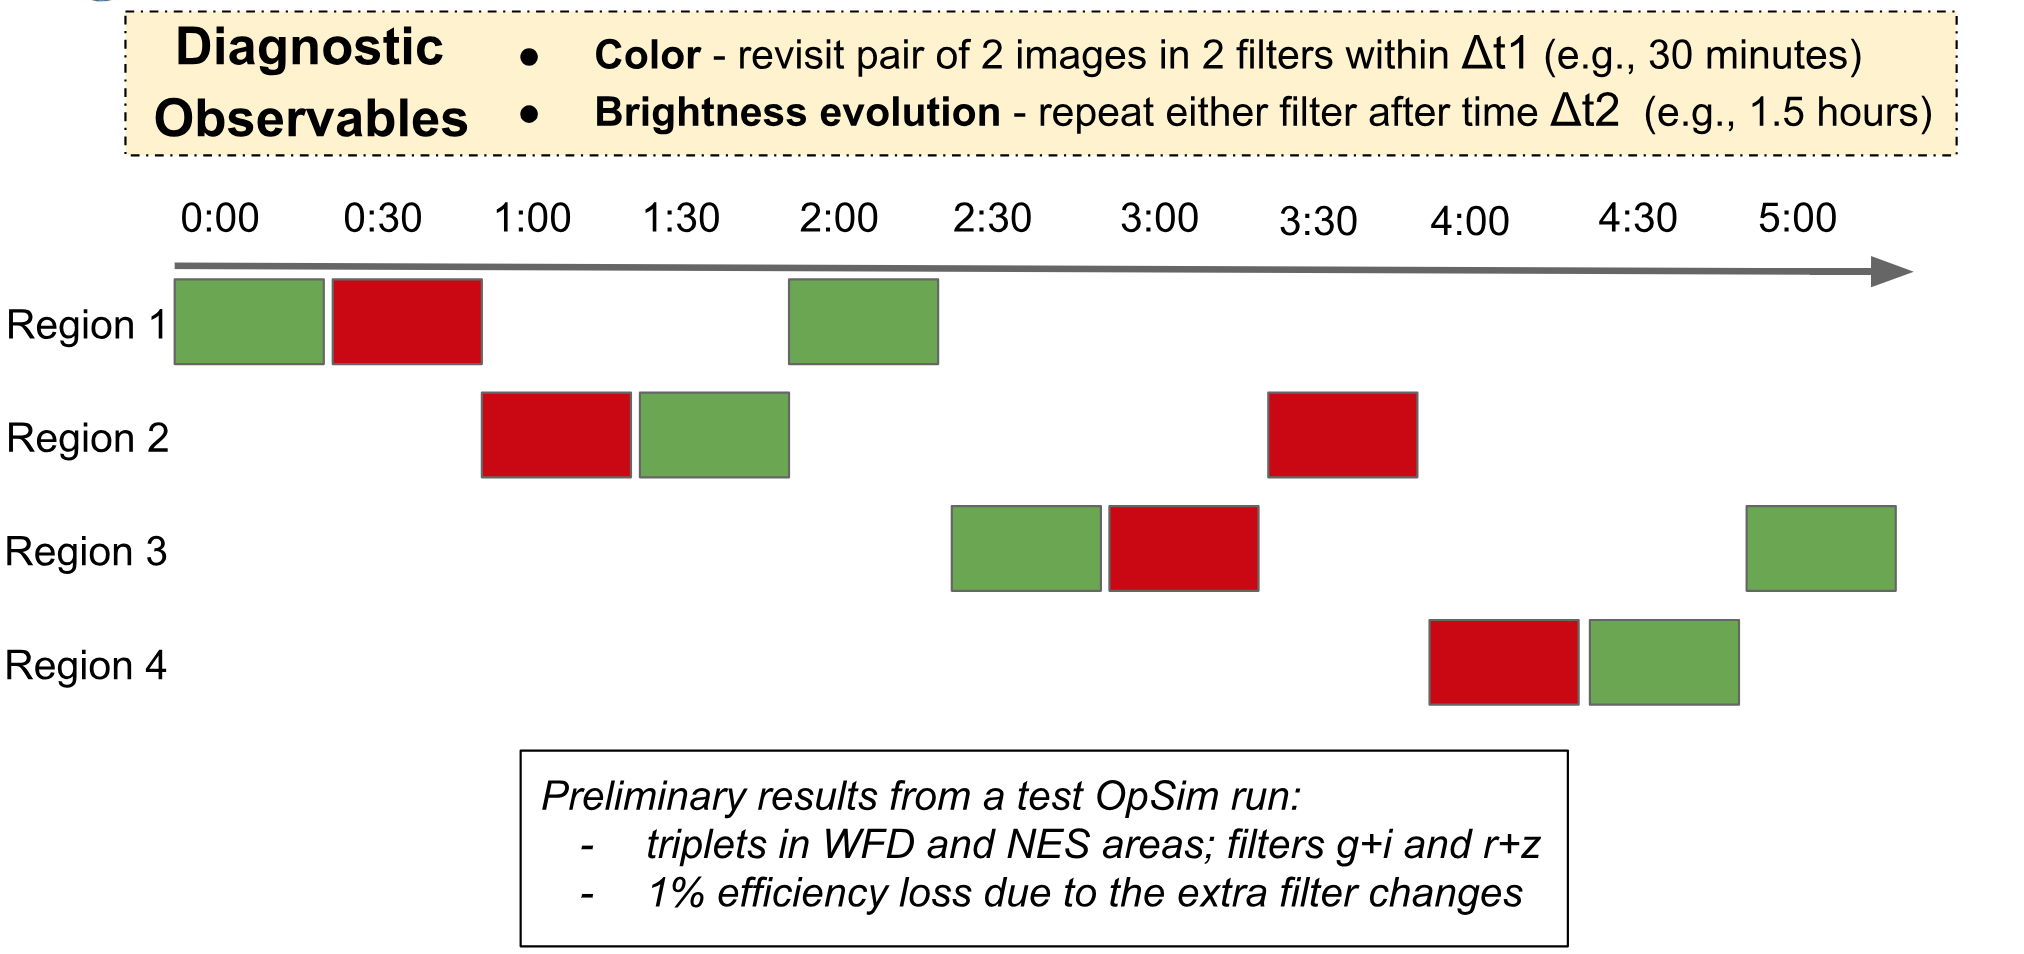
\includegraphics[width=0.9\textwidth]{figures/highLevelCadence.png}
\caption{{\footnotesize An example {\em Presto-Color} cadence with two alternating filters cover regions of sky to obtain three observations per region with appropriate time gaps to measure lightcurve color and shape.}}
\end{figure}

\subsection{Footprint -- pointings, regions and/or constraints}
%\begin{footnotesize}{\it Describe the specific pointings or general region (RA/Dec, Galactic longitude/latitude or Ecliptic longitude/latitude) for the observations. Please describe any additional requirements, especially if there are no specific constraints on the pointings (e.g. stellar density, galactic dust extinction).}
%\end{footnotesize}

\noindent This proposed cadence does not make any additional constraints on the imaging area compared to WFD. The science goals might be reachable if the proposed cadence was implemented over a sub-region of the WFD survey area. As the change of filters in the first pair of observations may limit the detectability of Solar System objects (to the magnitude depth of the shallower filter) this survey strategy could be implemented only in a subset of filters on the extended ecliptic plane (the region of interest for Solar System detections).

\subsection{Image quality}
%\begin{footnotesize}{\it Constraints on the image quality (seeing).}\end{footnotesize}

\noindent This proposed cadence does not make any additional constraints on the image quality compared to WFD. 

\subsection{Individual image depth and/or sky brightness}
%\begin{footnotesize}{\it Constraints on the sky brightness in each image and/or individual image depth for point sources. Please differentiate between motivation for a desired sky brightness or individual image depth (as calculated for point sources). Please provide sky brightness or image depth constraints per filter.}
%\end{footnotesize}

\noindent This proposed cadence does not make any additional constraints on the individual image depth or sky brightness compared to WFD. 


\subsection{Co-added image depth and/or total number of visits}
%\begin{footnotesize}{\it  Constraints on the total co-added depth and/or total number of visits. Please differentiate between motivations for a given co-added depth and total number of visits. Please provide desired co-added depth and/or total number of visits per filter, if relevant.}
%\end{footnotesize}

\noindent This proposed cadence does not make any additional constraints on the co-added image depth or total number of visits compared to WFD. 


\subsection{Number of visits within a night}
%\begin{footnotesize}{\it Constraints on the number of exposures (or visits) in a night, especially if considering sequences of visits.}
%\end{footnotesize}

\noindent The proposed cadence requires at least 3 visits per night.

\subsection{Distribution of visits over time}
%\begin{footnotesize}{\it Constraints on the timing of visits --- within a night, between nights, between seasons or between years (which could be relevant for rolling cadence choices in the WideFastDeep. Please describe optimum visit timing as well as acceptable limits on visit timing, and options in case of missed visits (due to weather, etc.). If this timing should include particular sequences of filters, please describe.}
%\end{footnotesize}

We require three total observations in a night in 2 total filters. The 2 observations in different filters are separated by \dtone\ minutes, and will be used to assess the color of the transient. As the physical processes operating depend on the \emph{intrinsic} color of the---potentially rapidly-evolving---transients, smaller values of \dtone\ on the order of $\sim$30 minutes are preferred. However, \dtone\ values up to a few hours, while no longer sensitive to the true color of the transient at a given moment, still provide diagnostic power of whether a given transient is red or blue, and will therefore allow us to achieve some of our science goals.

In addition, a second observation should be obtained in \emph{either} one of the two filter separated in time by \dttwo\ minutes. This observation can be obtained either \emph{before or after} the filter pair, and will be used to measure the light curve slope. Longer intra-night separations on the order of $\sim$4$-$5 hours are preferred, as our transients of interest distinguish themselves from longer-lived supernova at higher signal-to-noise over these timescales (Fig 2). Shorter \dttwo\ separations of $\sim$1.5 hours will still allow us to achieve some of our science goals, as very young supernovae and rapidly-rising transients evolve at $>$0.1 mag/hour. However, on these shorter timescales most currently known rapidly-declining transients will evolve by only $\sim$0.02$-$0.03 mag, hindering their identification (Figure~2).   
We note that a non-detection in the isolated observation or the detection above the saturation limit would still provide constraints on the lightcurve evolution. However, a non-detection would provide some limited constraints on color.

Finally, we note that the science goals which motivate {\em Presto-Color} -- namely, well-characterized light curves for rapid events -- have overlap with the science motivations of a rolling cadence. This proposed cadence would benefit from being implemented in regions where rolling cadence is applied (i.e., an intra-night gap $<3$ days).


\subsection{Filter choice}
%\begin{footnotesize}
%{\it Please describe any filter constraints not included above.}
%\end{footnotesize}

\noindent Filters should be pair. For the fast transients under consideration the preferred filter pairs are  $g-i$ or $r-z$ as non-adjacent pairs provide a larger lever arm for distinguishing a given transient as red or blue. In particular, many infant supernova rapidly-rising transients can be very blue at early times, favoring the inclusion of the $g-$ (or $r-$) band. However, we emphasize that some of our science can be be achieved with any filter pair.

%it appears that non-adjacent filter pairs 
%that skip the in-between filter in the sequence are optimal for our science.   

%with a gap in the sequence

\subsection{Exposure constraints}
%\begin{footnotesize}
%{\it Describe any constraints on the minimum or maximum exposure time per visit required (or alternatively, saturation limits). Please comment on any constraints on the number of exposures in a visit.}
%\end{footnotesize}

\noindent This proposed cadence uses the baseline exposure times of $2\times15$ seconds or $1\times30$ seconds. $2\times15$ seconds is a preferred snap strategy, since in case of saturation of these {\em rapidly evolving transients} constraints a reliable magnitude measurement could be obtained from the individual snaps.

\subsection{Other constraints}
%\begin{footnotesize}
%{\it Any other constraints.}
%\end{footnotesize}

\noindent We propose that {\em Presto-Color} be implemented on extragalactic fields, but note that it may also be useful in some Galactic Plane fields to detect and characterize microlensing events on short timescales, binary stars, and black holes, for example. Trade-offs and synergies with other proposals are discussed further in Section 3.12, Item 5.


\subsection{Estimated time requirement}
%\begin{footnotesize}
%{\it Approximate total time requested for these observations, using the guidelines available at \url{https://github.com/lsst-pst/survey_strategy_wp}.}
%\end{footnotesize}

\noindent Since our proposed cadence is a modification of the WFD strategy -- a shuffling of the visits, not adding visits -- we are not requesting that any additional time be added to the WFD component. However, as mentioned in Section~\ref{sec:item:category}, {\em Presto-Color} could be implemented as a mini-survey instead of as part of WFD. For example, if the majority of $g$-band visits in the WFD survey are uniformly distributed in time, with paired visits in $i$-band within a time of \dtone, then a mini-survey which adds $g$- or $i$-band visits within time \dttwo\ could be implemented to meet our science goals. This option would be within the $\sim 1\% $ time requirement for mini-surveys if, for example, it is restricted to areas of $1800$ sq. degrees for 10 years, or covers the full $18000$ sq degrees for a single year.

\vspace{.3in}

\begin{table}[ht]
    \centering
    \begin{tabular}{|l|l|l|l}
        \toprule
        Properties & Importance \hspace{.3in} \\
        \midrule
        Image quality &   3  \\
        Sky brightness &  3\\
        Individual image depth & 3  \\
        Co-added image depth &   3\\
        Number of exposures in a visit   &  3 \\
        Number of visits (in a night)  &  1 \\ 
        Total number of visits &   3\\
        Time between visits (in a night) & 1 \\
        Time between visits (between nights)  & 2  \\
        Long-term gaps between visits & 3\\
        Other \emph{filter pairs within night} & 1 \\
        \bottomrule
    \end{tabular}
    \caption{{\bf Constraint Rankings:} {\em Presto-Color} has strict requirements on the filter selection, number of visits per night, and the intra-night revisit time gaps. The science case would benefit from a shorter inter-night gap, because additional observations at a $\sim$day time scale (in the nights following detection) would help to both refine the follow-up strategy, and collect survey data that could be used in photometric sample studies based on the LSST data alone. Since the transients of interest are predominantly blue, this proposal would prioritize visits in the $g$-band filter.}.
    % I think it is worth mentioning this somewhere in the paper. g band has 80 visits per field in 10 years compared to r ~ 184, i ~184, z, y ~ 160.  
        \label{tab:obs_constraints}
\end{table}

\subsection{Technical trades}
%{\footnotesize {\it To aid in attempts to combine this proposed survey modification with others, please address the following questions:}}
\begin{enumerate}
    \item {\footnotesize {\it What is the effect of a trade-off between your requested survey footprint (area) and requested co-added depth or number of visits?}} \\ As with a rolling cadence, the area in which this {\em Presto-Color} strategy is applied will lower the visit cadence in other areas, but need not affect the total number of visits per field or the final co-added depths of the WFD survey.
    \item {\footnotesize {\it If not requesting a specific timing of visits, what is the effect of a trade-off between the uniformity of observations and the frequency of observations in time? e.g. a `rolling cadence' increases the frequency of visits during a short time period at the cost of fewer visits the rest of the time, making the overall sampling less uniform.}} \\ As with a rolling cadence, during the time when a field is not within the area being covered by the {\em Presto-Color} strategy, it will receive fewer visits.
    \item {\footnotesize {\it What is the effect of a trade-off on the exposure time and number of visits (e.g. increasing the individual image depth but decreasing the overall number of visits)?}} \\ Discovering and characterizing fast transients and fast features does not benefit from increasing in exposure time at the expense of the number of visits. Increasing the number of visits at the expense of exposure time might benefit our program a bit, but much shorter exposures could increase the uncertainty of slopes and colors measured from two visits. 
    \item {\footnotesize {\it What is the effect of a trade-off between uniformity in number of visits and co-added depth? Is there any benefit to real-time exposure time optimization to obtain nearly constant single-visit limiting depth?}} \\ The science goals that motivate the {\em Presto-Color} strategy do not benefit from increased co-added depth or maintaining a constant single-visit limiting depth.
    \item {\footnotesize {\it Are there any other potential trade-offs to consider when attempting to balance this proposal with others which may have similar but slightly different requests?}}  
    
    There are a few other cadence proposals similar to the {\em Presto-Color} strategy. We discuss similarities and trade-offs for each in turn:  
    
    {\bf \emph{(1) Street et al. ``The Diverse Science Return from a Wide-Area Survey of the Galactic Plane"}}, which proposes the ``paired-$i$" strategy: fields in the Galactic plane are imaged every 2-3 days, first in $i$-band and then 1-4 hours later a revisit in $g$, $r$, or $z$. The basic motivation is the same -- to identify rapidly varying transients and characterize them via colors -- just for Galactic variables like Young Stellar Objects and Cataclysmic Variables. However, since we propose the {\em Presto-Color} strategy for the extragalactic WFD there is no tension between these two white papers. 
    
    {\bf \emph{(2) Bricman et al. ``TDEs with LSST"}}, proposes to get same-night color information. The version that we read requested to change the filter between the two $15$-second exposures of a visit, which isn't possible, but we surmised that what they actually want is for two visits in a night in two different filters. If so, then this {\em Presto-Color} proposal would also suite their needs. 
    
    {\bf \emph{(3) Gezari et al. ``An Extreme Rolling Cadence Wide-Fast-Deep Survey"}}, proposes to do the full WFD area in only years 1 and 10, and rotate through 8 equal strips of area in years 2 through 9. While this would often result in 2-3 visits per night, probably in multiple filters, no specific filter pairings or revisit timescales are requested. The trade-off between these proposals is that such an extreme rolling cadence would remove the opportunity for longer-term monitoring of transients with fast features, such as Type IIn SNe, which can last for years.  
\end{enumerate}


\clearpage
%%%%%%%%%%%%%%%%%%%%%%%%%%%%%%%%%%%%%%%%%%%%%%%%%%%
\section{Performance Evaluation}
%\begin{footnotesize}
%{\it Please describe how to evaluate the performance of a given survey in achieving your desired science goals, ideally as a heuristic tied directly to the observing strategy (e.g. number of visits obtained within a window of time with a specified set of filters) with a clear link to the resulting effect on science. More complex metrics which more directly evaluate science output (e.g. number of eclipsing binaries successfully identified as a result of a given survey) are also encouraged, preferably as a secondary metric. If possible, provide threshold values for these metrics at which point your proposed science would be unsuccessful and where it reaches an ideal goal, or explain why this is not possible to quantify. While not necessary, if you have already transformed this into a MAF metric, please add a link to the code (or a PR to \href{https://github.com/lsst-nonproject/sims_maf_contrib}{sims\_maf\_contrib}) in addition to the text description. (Limit: 2 pages).}
%\end{footnotesize}

\subsection{Diagnostic Metrics}

Based on our evaluation of the light curves of fast transients, and the fast features of longer duration transients, we designed 2 diagnostic metrics and submitted them to the {\em sims\_maf\_contrib } repository.

\begin{enumerate}
\vspace{-0.15in}
\item
{\bf threeVisitsWColorMetric}: a {\it diagnostic} metric that checks if a field was observed 3 times in a night with 2 filters, given input constraints on \dtone\ (an upper limit) and \dttwo\ (a lower limit). The specific filter pair of $f_1$ and $f_2$ is also an input to the metric. This metric was run on year 1 of {\tt baseline2018a} and year 1 of our test {\tt OpSim} run {\tt pontus\_2591}. Results are shown and discussed in Figure~4.
\item
\vspace{-0.1in}
{\bf FastTransientMetric}: a {\it diagnostic} metric based on the {\tt Transient Metric} that injects continuous saw-tooth shaped transients with a rising slope (input parameter) and a vertical decline, with input peak brightness which can be input independently for each filter (thus enabling the injection of different color transients). The metric calculates the fraction of transients with three detections that are consistent with an input \dtone\ (upper limit) and \dttwo\ (lower limit) and a specific filter-pair.

\end{enumerate}
\vspace{-0.2in}

\subsection{Figure of Merit Metric}

Our Figure of Merit (FoM) metric is the fraction of events for which the color and rise-time are constrained (within some accuracy). Different science cases will have different input lightcurves and different gap constraints. We plan on injecting samples of the transients of interest, as well as ``normal" transients, by leveraging the Monte Carlo MAF framework and the {\tt transientLC} metric, recovering the lightcurve ({\tt PassMetric}) and measuring color and slope, which will be evaluated in the context of  machine learning partitioning of the Color-Slope phase space (Figure 2) to isolate transients for follow-up. Further analysis will assess our ability to distinguish between fast transients with the LSST data alone.


\subsection{Create OpSim}

{\tt OpSim} runs using the new feature based scheduler are being created. The {\em Presto-Color} survey strategy is accomplished with a combination of the {\it Greedy Algorithm} (GA Survey), {\it Pairs in different filters} (PDF Survey) and {\it Pairs in the same filters} (PSF Survey) Surveys. To combine observations in filters $f_1$ and $f_2$, the Surveys are configured such that when the {\it GA Survey} in $f_1$ or $f_2$ gets an observation, the {\it PDF Survey} schedules an observation of the same field with the other filter $30 \pm 5$ min later, and the {\it PSF Survey} scheduler an observation of the same field with the same filter $60 \pm 5$ min later. A test simulation combining $gi$ and $rz$ was produced to evaluate the impact in performance and test the metrics. Non-adjacent filters are used to get a better leverage on the Spectral Energy Distribution (SED) color. Overall we noticed that this kind of strategy has a similar throughput (in efficiency and total number of observations) as a strategy to take pairs of observations in different filters. 

% that perform $f_1$ observations on a field, 30 min later repeat the pointing pattern in $f_2$, and 60 min later repeat the pointing pattern in $f_1$ or $f_2$, where $f_1$ and $f_2$ are $g$ and $i$, or $r$ and $z$. 

\begin{figure}[!ht]
\begin{center}
% \begin{subfigure}[b]{1.0\textwidth}
% \includegraphics[width=5cm,height=4cm]{figures/3visits_pontus_2564_gi.png}
% \includegraphics[width=5cm,height=4cm]{figures/3visits_pontus_2564_rz.png}
% \includegraphics[width=5cm,height=4cm]{figures/3visits_pontus_2564_grgzriiz.png}
% \end{subfigure}
% \begin{subfigure}[b]{1\textwidth}
% 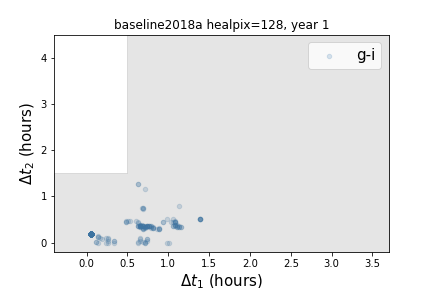
\includegraphics[width=5cm,height=4cm]{figures/3visits_baseline2018a_gi.png}
% 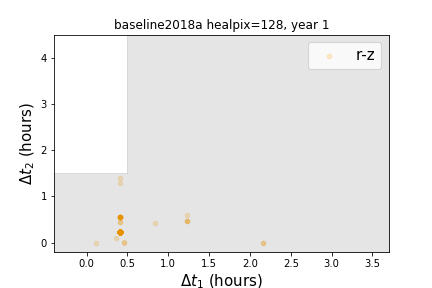
\includegraphics[width=5cm,height=4cm]{figures/3visits_baseline2018a_rz.png}
% 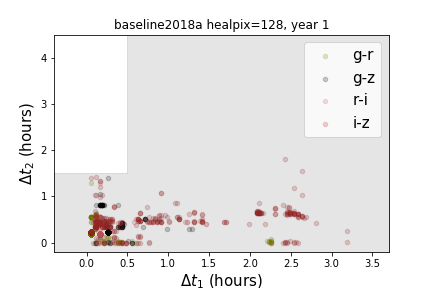
\includegraphics[width=5cm,height=4cm]{figures/3visits_baseline2018a_grgzriiz.png}
% \end{subfigure}
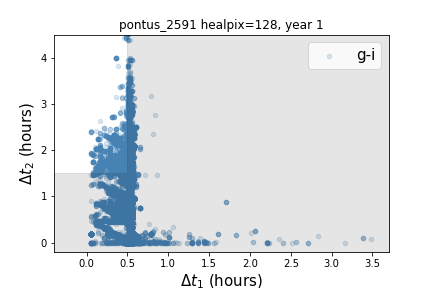
\includegraphics[width=6.5cm,height=5cm]{figures/3visits_pontus_2591_gi.png}
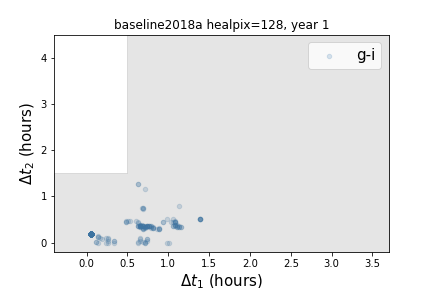
\includegraphics[width=6.5cm,height=5cm]{figures/3visits_baseline2018a_gi.png}
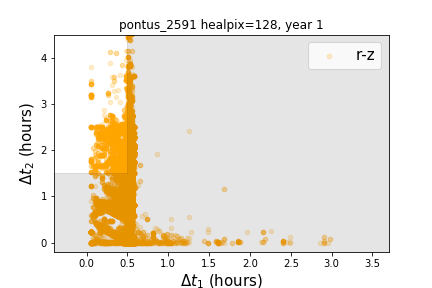
\includegraphics[width=6.91cm,height=5cm]{figures/3visits_pontus_2591_rz.png}
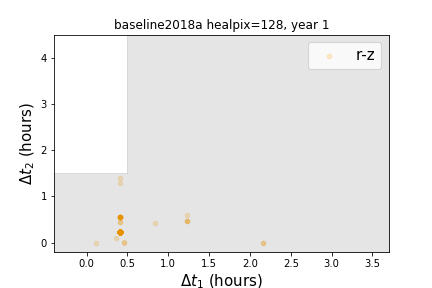
\includegraphics[width=6.5cm,height=5cm]{figures/3visits_baseline2018a_rz.png}
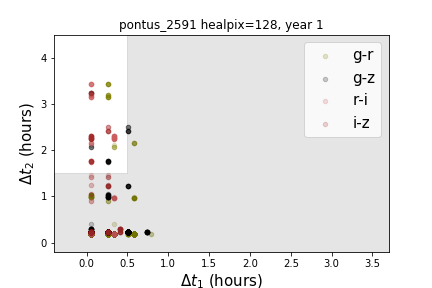
\includegraphics[width=6.5cm,height=5cm]{figures/3visits_pontus_2591_grgzriiz.png}
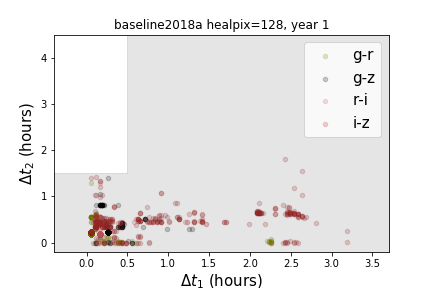
\includegraphics[width=6.5cm,height=5cm]{figures/3visits_baseline2018a_grgzriiz.png}
\caption{{\footnotesize The results of our {\em diagnostic} metric, {\tt threeVisitsWColorMetric}, that checks for fields that were observed 3 times in a night with 2 filters (as labeled) satisfying the constraints on \dtone\ and \dttwo. We show results for 1-year of {\tt pontus\_2591} (our {\em Presto-Color} test run; left), and {\tt baseline2018a} LSST observations (right). All {\tt HEALpix} ``fields" that met the conditions of our metric are shown as points, colored by the filter pair $f_1$-$f_2$. The $x-$axis is the time between visits in the two different filters (which provide color; \dtone), and the $y-$axis is the time between visits in the same filter (which provides slope; \dttwo). The target area for our science is the white region, where $\dtone<0.5$ and $\dttwo>1.5$ hours, such that both color and brightness evolution can be measured, although there is no hard cutoff at 30 minutes in \dtone, so observations just to the left of our target region are valuable, and observations at a larger \dttwo~ within the same night are preferred.
%: this area provides constraints on the color, in spite of the fast color evolution of some of our targeted transients, as well as constraints on the slope that enable us to distinguish fast-evolving transients from "normal" transients (e.g. SN\,Ia).
In {\tt pontus\_2591} 20 thousand observations in year 1 satisfy our constraints strictly ($\dtone<0.5$ and $\dttwo>1.5$) in $g-i$ and over 40 thousand in $r-z$.
Very few {\tt HEALpix} fields in the {\tt baseline2018a} {\tt OpSim} have observations in triplets in 2 filters and none that satisfy our constraints.}}
\end{center}
\end{figure}

\vspace{.6in}

\clearpage
%%%%%%%%%%%%%%%%%%%%%%%%%%%%%%%%%%%%%%%%%%%%%%%%%%%
\section{Special Data Processing}
%\begin{footnotesize}
%{\it Describe any data processing requirements beyond the standard LSST Data Management pipelines and how these will be achieved.}
%\end{footnotesize}

The science goals that motivate the proposed {\em Presto-Color} cadence will not require any special data processing; the planned Prompt and Data Release pipelines and their data products will be sufficient for our science goals. 

\section{Acknowledgments}
This work was developed within the Transients and Variable Stars Science Collaboration (TVS) and the author acknowledges the support of TVS in the preparation of this paper. 

\noindent
The authors acknowledge support by the Flatiron Institute and Heising-Simons Foundation for the development of this paper.

%%%%%%%%%%%%%%%%%%%%%%%%%%%%%%%%%%%%%%%%%%%%%%%%%%%
\bibliographystyle{aasjournal}
%\bibliographystyle{ieeetr}

\bibliography{main}

\end{document}
